% Section content template for individual Educative lessons
% This file contains the actual content for a specific section
% Generated from Educative API section content

% Section: Design of a Pub-Sub System
% Section ID: 5367894619193344
% Section Slug: design-of-a-pub-sub-system
% Generated: 2025-12-07T21:18:04.337101

\subsection{First design}\label{Iu3pxhyrG3uS_5Reopgel}
\\
In the previous lesson, we discussed that a producer writes into topics, and consumers subscribe to a topic to read messages from that topic. Since new messages are added at the end of the queue, we can use \href{https://www.educative.io/courses/grokking-the-system-design-interview/system-design-the-distributed-messaging-queue}{distributed messaging queues} for topics.
\\
The components we'll need have been listed below:

\begin{itemize}
\item
\protect\phantomsection\label{oEck4F-0mAyITc5flQmUN}
\textbf{Topic queue}: Each topic will be a distributed messaging queue so we can store the messages sent to us from the producer. A producer will write their messages to that queue.
\item
\protect\phantomsection\label{MehSUdTCHXSrN44TOeaY1}
\textbf{Database}: We'll use a relational database that will store the subscription details. For example, we need to store which consumer has subscribed to which topic so we can provide the consumers with their desired messages. We'll use a relational database since our consumer-related data is structured and we want to ensure our data integrity.
\item
\protect\phantomsection\label{eLzpa_um2ZjTL7zavE1Ux}
\textbf{Message director}: This service will read the message from the topic queue, fetch the consumers from the database, and send the message to the consumer queue.
\item
\protect\phantomsection\label{WyuLhMmYaTf2JKndcDAwT}
\textbf{Consumer queue}: The message from the topic queue will be copied to the consumer's queue so the consumer can read the message. For each consumer, we'll define a separate distributed queue.
\item
\protect\phantomsection\label{H-00xmG48Ov1yj9VIo2AJ}
\textbf{Subscriber}: When the consumer requests a subscription to a topic, this service will add an entry into the database.
\end{itemize}
\\
The consumer will subscribe to a topic, and the system will add the subscriber's details to the database. The producer will write into the topics, and the message director will read the message from the queue, fetch the details to whom it should add the message, and send it to them. The consumers will consume the message from their queue.
\begin{quote}
\textbf{Note}: We'll use fail-over services for the message director and subscriber to guard against failures.
\end{quote}

\begin{figure}[htbp]
 \centering
 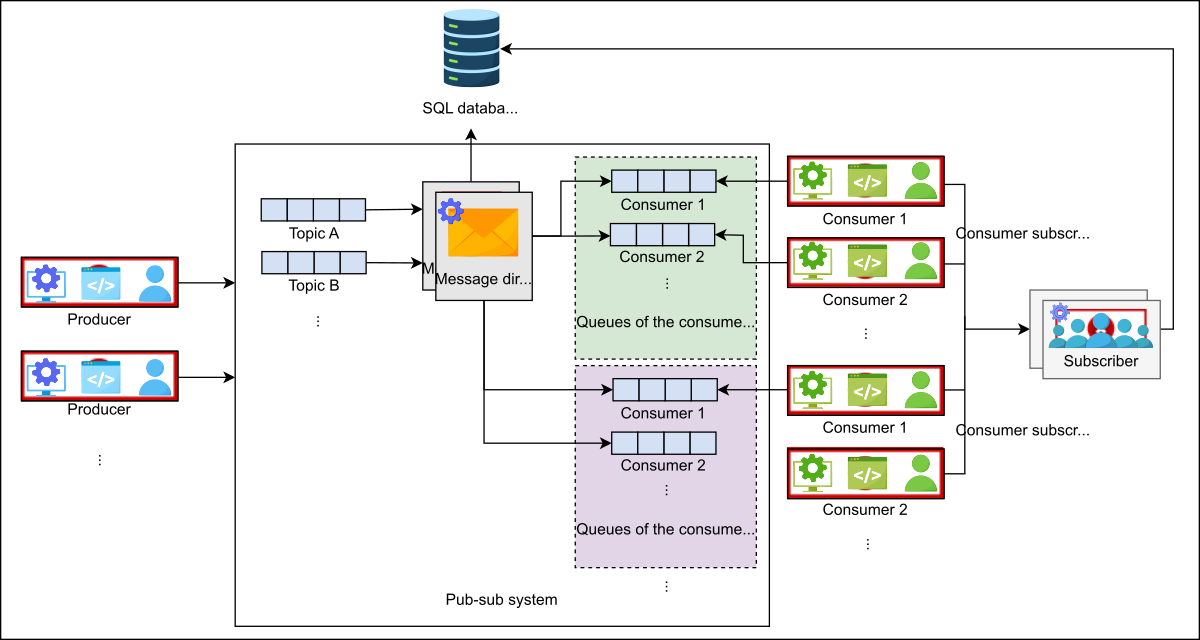
\includegraphics[width=0.5\textwidth]{Images/chapter_18/section_5367894619193344/4935815550861312.png}
 \caption{Using the distributed messaging queue}
\end{figure}

Using the distributed messaging queues makes our design simple. However, the huge number of queues needed is a significant concern. If we have millions of subscribers for thousands of topics, defining and maintaining millions of queues is expensive. Moreover , we'll copy the same message for a topic in all subscriber queues, which is unnecessary duplication and takes up space.

\begin{quote}
\textbf{Quiz:}
\textbf{Question 1:} Is there a way to avoid maintaining a separate queue for each reader?
\textbf{Answer:} In messaging queues, the message disappears after the reader consumes it. So, what if we add a counter for each message? The counter value decrements as a subscriber consumes the message. It does not delete the message until the counter becomes zero. Now, we don't need to keep a separate queue for each reader.
\textbf{Question 2:} What is the problem with the previous approach?
\textbf{Answer:} The unread messages can become a bottleneck if we use the conventional queue API. For example, if 9 out of 10 readers have consumed the message present at the start of the queue, then that message won't be deleted until the tenth consumer has also consumed the message, and the first nine consumers won't be able to move forward. We'll need to change the storage interface so that consumers can independently consume data. Our system will need to keep sufficient metadata and track what information each consumer has consumed and delete a message when the information has been consumed by all consumers. It resembles with reference count mechanism in Linux\textquotesingle s hard link of files.
\end{quote}

\subsection{Second design}\label{nwbvqM9Ct2Ll2eWXtUtWA}
\\
Let's consider another approach to designing a pub-sub system.

\subsubsection{High-level design}\label{2LCZMS7RMXLiMFKKDcrnn}
\\
At a high level, the pub-sub system will have the following components:

\begin{itemize}
\item
\protect\phantomsection\label{zvW4TXnsp6DDTxHLt5M-b}
\textbf{Broker}: This server will handle the messages. It will store the messages sent from the producer and allow the consumers to read them.
\item
\protect\phantomsection\label{uiLmc3ppJlYay6i_vUCk2}
\textbf{Cluster manager}: We'll have numerous broker servers to cater to our scalability needs. We need a cluster manager to supervise the broker's health. It will notify us if a broker fails.
\item
\protect\phantomsection\label{2-Bw-8FuPeh5MnROirf5l}
\textbf{Storage}: We'll use a relational database to store consumer details, such as subscription information and retention period.
\item
\protect\phantomsection\label{fdeN-Go2A3JiEryPxmcGa}
\textbf{Consumer manager}: This is responsible for managing the consumers. For example, it will verify if the consumer is authorized to read a message from a certain topic or not.
\end{itemize}
\\
Besides these components, we also have the following design considerations:

\begin{itemize}
\item
\protect\phantomsection\label{DUrVeIhHobX3vrzt2BoRn}
\textbf{Acknowledgment}: An acknowledgment is used to notify the producer that the received message has been stored successfully. The system will wait for an acknowledgment from the consumer if it has successfully consumed the message.
\item
\protect\phantomsection\label{kiPuFpVyK9Px4bntsBmdP}
\textbf{Retention time}: The consumers can specify the retention period time of their messages. The default will be seven days, but it is configurable. Some applications like banking applications require the data to be stored for a few weeks as a business requirement, while an analytical application might not need the data after consumption.
\end{itemize}

\begin{figure}[htbp]
 \centering
 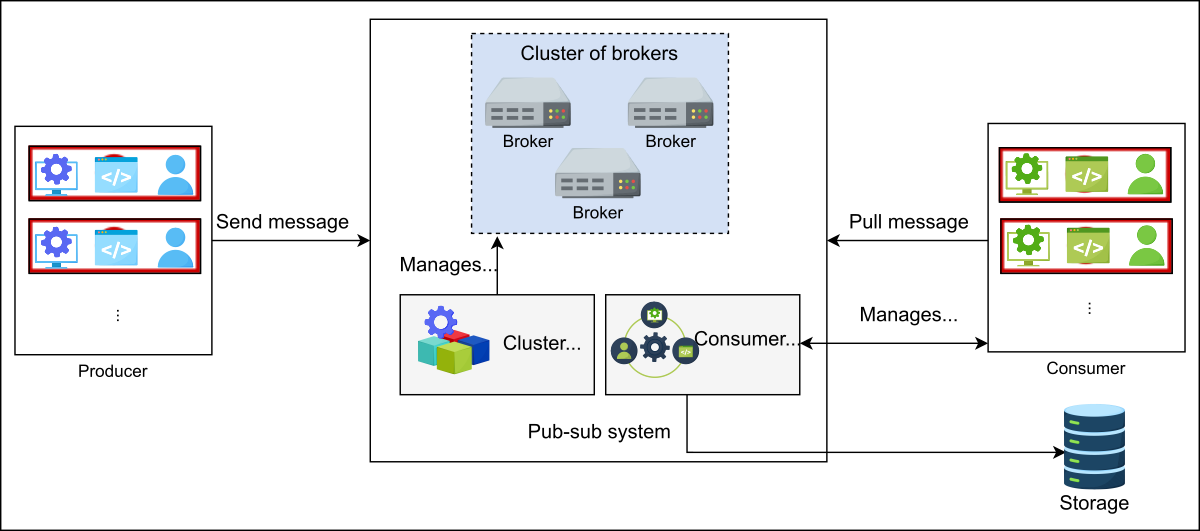
\includegraphics[width=0.5\textwidth]{Images/chapter_18/section_5367894619193344/6475504921477120.png}
 \caption{High-level design of a pub-sub system}
\end{figure}

Let's understand the role of each component in detail.

\subsection{Broker}\label{lnwomSuVIbDKxiKeYBcPr}
\\
The broker server is the core component of our pub-sub system. It will handle write and read requests. A broker will have multiple topics, where each topic can have multiple \textbf{partitions} associated with it. We use partitions to store messages in the local storage for persistence. Consequently, this improves availability. Partitions contain messages encapsulated in \textbf{segments}.
\\
Segments help identify the start and end of a message using an offset address. Using segments, consumers consume the message of their choice from a partition by reading from a specific offset address. The illustration below depicts the concept that has been described above.

\begin{figure}[htbp]
 \centering
 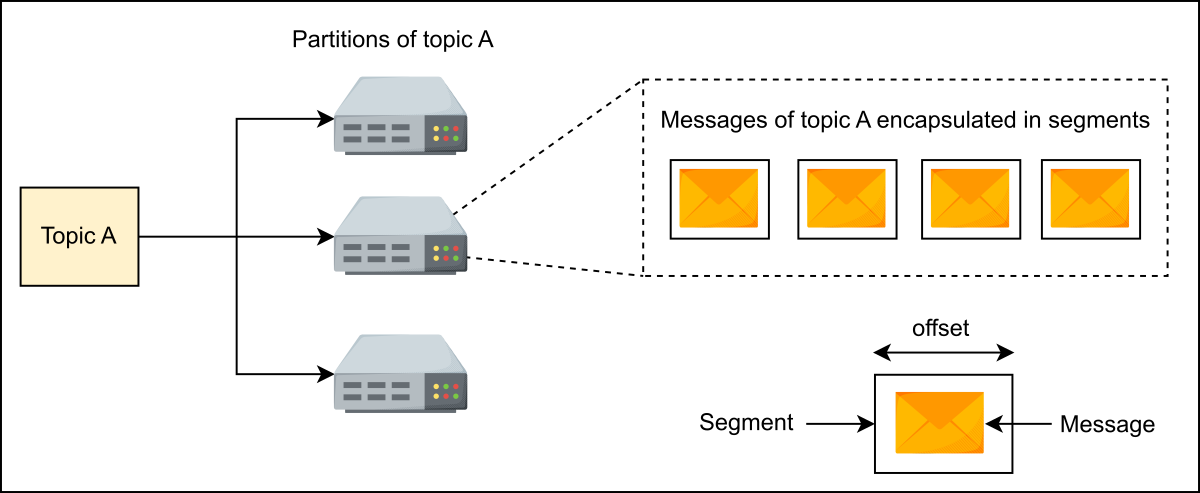
\includegraphics[width=0.5\textwidth]{Images/chapter_18/section_5367894619193344/4615528054652928.png}
 \caption{A depiction of how messages are stored within segments inside a partition}
\end{figure}

As we know, a \textbf{topic} is a persistent sequence of messages stored in the local storage of the broker. Once the data has been added to the topic, it cannot be modified. Reading and writing a message from or to a topic is an I/O task for computers, and scaling such tasks is challenging. This is the reason we split the topics into multiple partitions. The data belonging to a single topic can be present in numerous partitions. For example, let's assume we have Topic A and we allocate three partitions for it. The producers will send their messages to the relevant topic. The messages received will be sent to various partitions on the basis of the round-robin algorithm(Round-robin is a simple and starvation-free CPU scheduling algorithm. In this algorithm, each process or job is given a fixed amount of time slice cyclically. Consider an example in which we have the time slice of 200 ms and a job whose execution time is 1000 ms. The operating system (OS) assigns the CPU to the task for 200 ms in the round-robin algorithm and then puts the job at the end of the scheduling queue. The other jobs in the queue are given equal time slices (200 ms each). This approach continues until all the jobs finish their execution.). We'll use a variation of round-robin: weighted round-robin(Weighted round robin is a generalization of round-robin scheduling. It serves a set of queues or tasks. Whereas round-robin cycles over the queues or tasks and gives one service opportunity per cycle, a weighted round-robin offers to each a fixed number of opportunities as specified by the configured weight, which serves to influence the portion of capacity received by each queue or task. In computer networks, a service opportunity is the emission of one packet if the selected queue is non-empty. Source: Wikipedia). The following slides show how the messages are stored in various partitions belonging to a single topic.

\begin{figure}[htbp]
 \centering
 \begin{subfigure}[b]{0.48\textwidth}
 \centering
 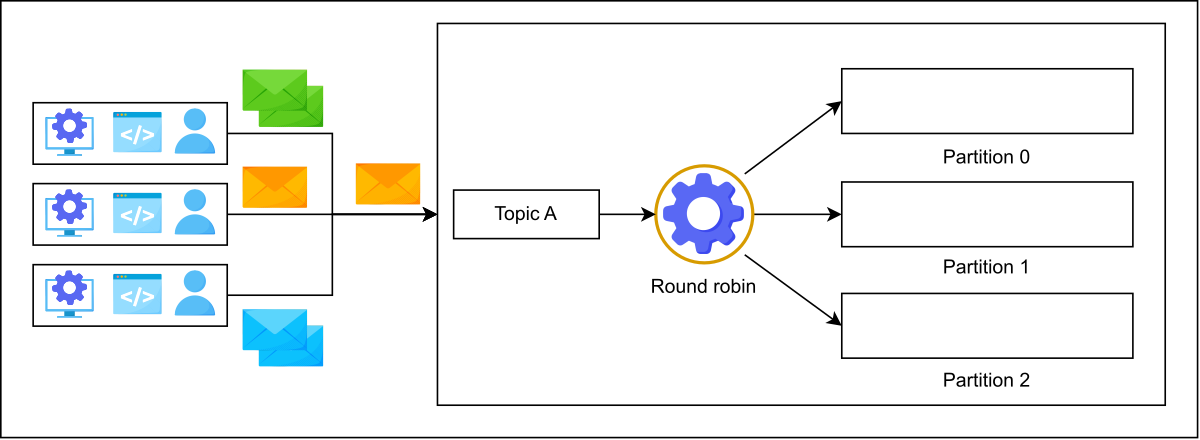
\includegraphics[width=\textwidth]{Images/chapter_18/section_5367894619193344/5964525213188096.png}
 \caption{The messages are added to the relative partitions.}
 \end{subfigure}
 \hfill
 \begin{subfigure}[b]{0.48\textwidth}
 \centering
 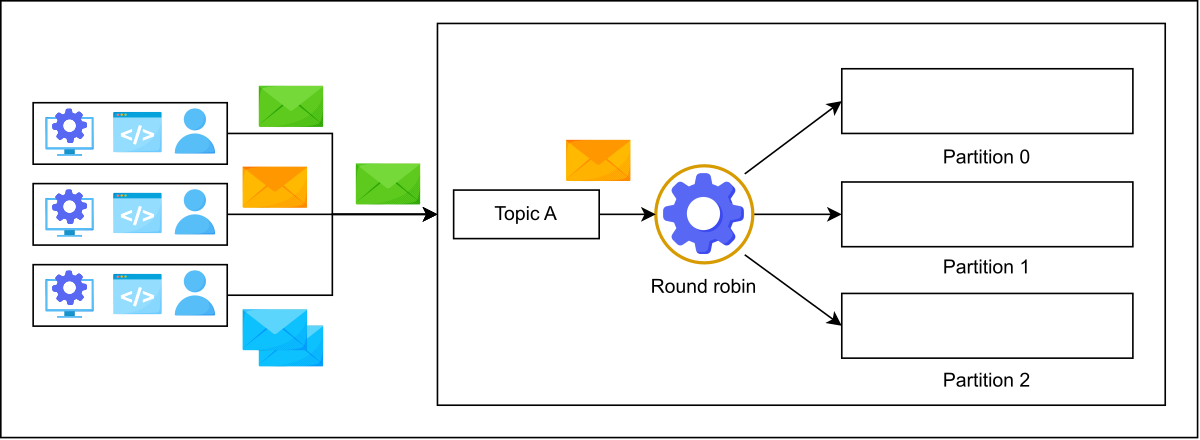
\includegraphics[width=\textwidth]{Images/chapter_18/section_5367894619193344/5621809774198784.png}
 \caption{The round-robin algorithm decides the partition where we need to store the message.}
 \end{subfigure}
\end{figure}

\begin{figure}[htbp]
 \centering
 \begin{subfigure}[b]{0.48\textwidth}
 \centering
 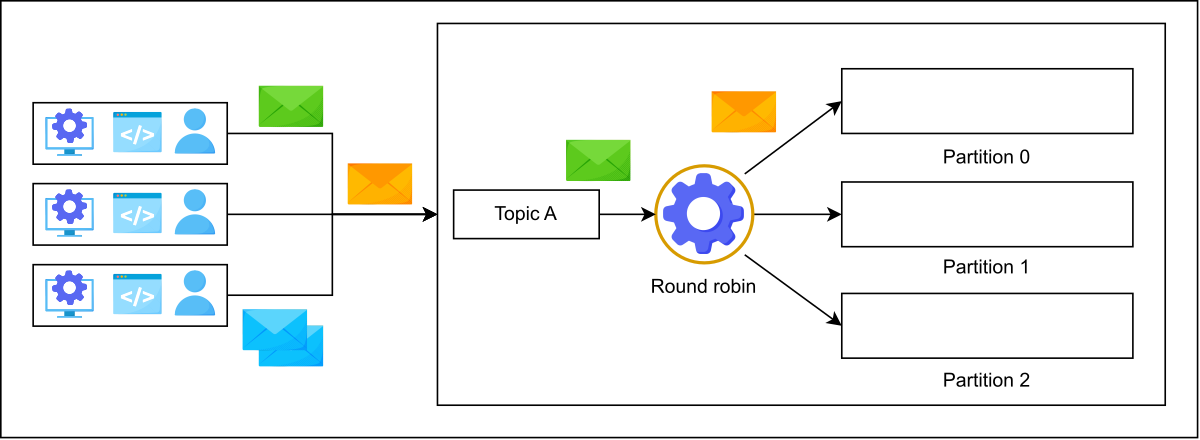
\includegraphics[width=\textwidth]{Images/chapter_18/section_5367894619193344/4635002702004224.png}
 \caption{The round-robin algorithm sends the message to Partition 0 and decides the partition for the incoming message.}
 \end{subfigure}
 \hfill
 \begin{subfigure}[b]{0.48\textwidth}
 \centering
 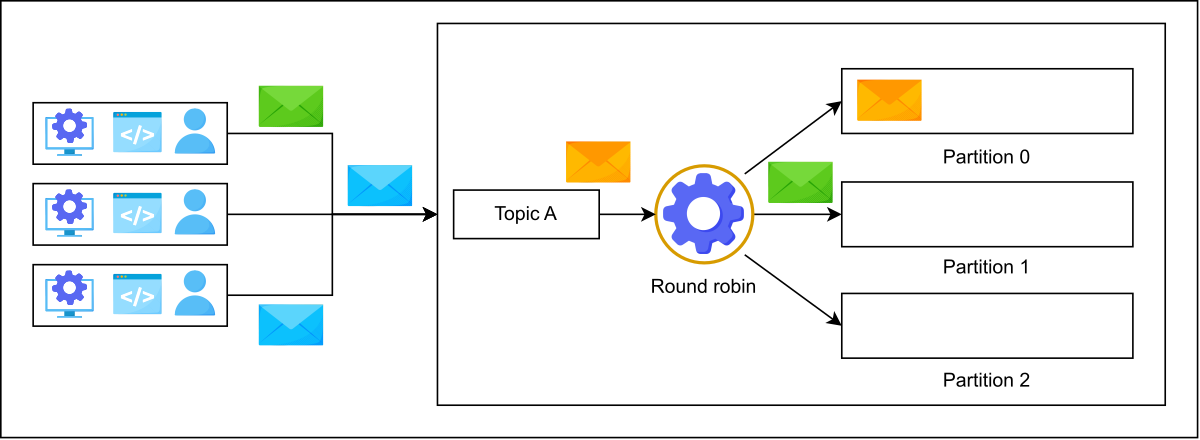
\includegraphics[width=\textwidth]{Images/chapter_18/section_5367894619193344/5668152202887168.png}
 \caption{The round-robin algorithm sends the message to Partition 1 and decides the partition for the incoming message.}
 \end{subfigure}
\end{figure}

\begin{figure}[htbp]
 \centering
 \begin{subfigure}[b]{0.48\textwidth}
 \centering
 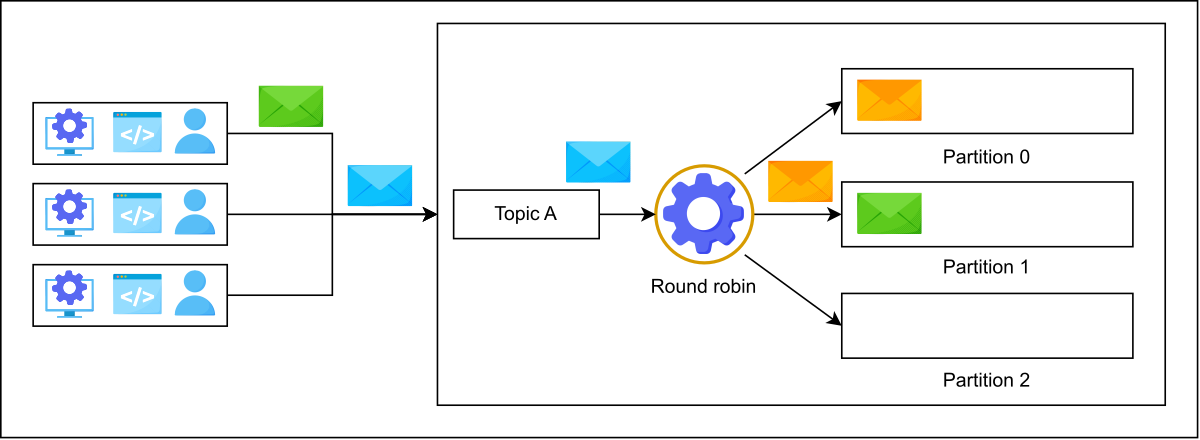
\includegraphics[width=\textwidth]{Images/chapter_18/section_5367894619193344/5448530308497408.png}
 \caption{The round-robin algorithm sends the message to Partition 1 and decides the partition for the incoming message.}
 \end{subfigure}
 \hfill
 \begin{subfigure}[b]{0.48\textwidth}
 \centering
 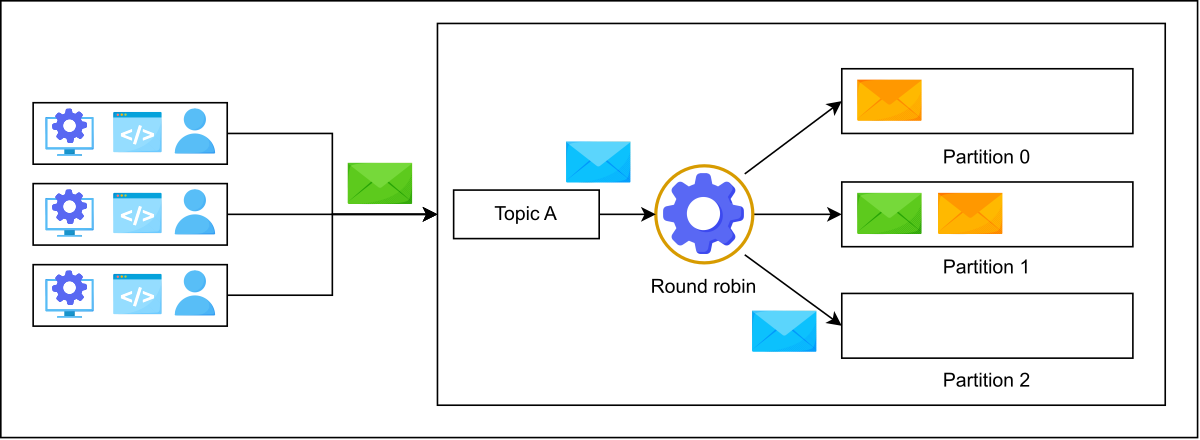
\includegraphics[width=\textwidth]{Images/chapter_18/section_5367894619193344/5852015004876800.png}
 \caption{The round-robin algorithm sends the message to Partition 2 and decides the partition for the incoming message.}
 \end{subfigure}
\end{figure}

\begin{figure}[htbp]
 \centering
 \begin{subfigure}[b]{0.48\textwidth}
 \centering
 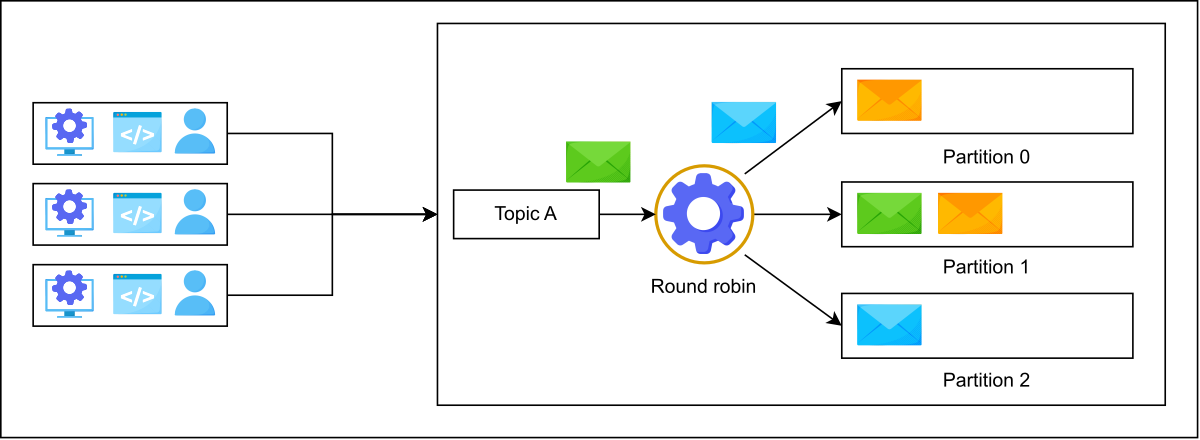
\includegraphics[width=\textwidth]{Images/chapter_18/section_5367894619193344/5215395675242496.png}
 \caption{The round-robin algorithm sends the message to Partition 0 and decides the partition for the incoming message.}
 \end{subfigure}
 \hfill
 \begin{subfigure}[b]{0.48\textwidth}
 \centering
 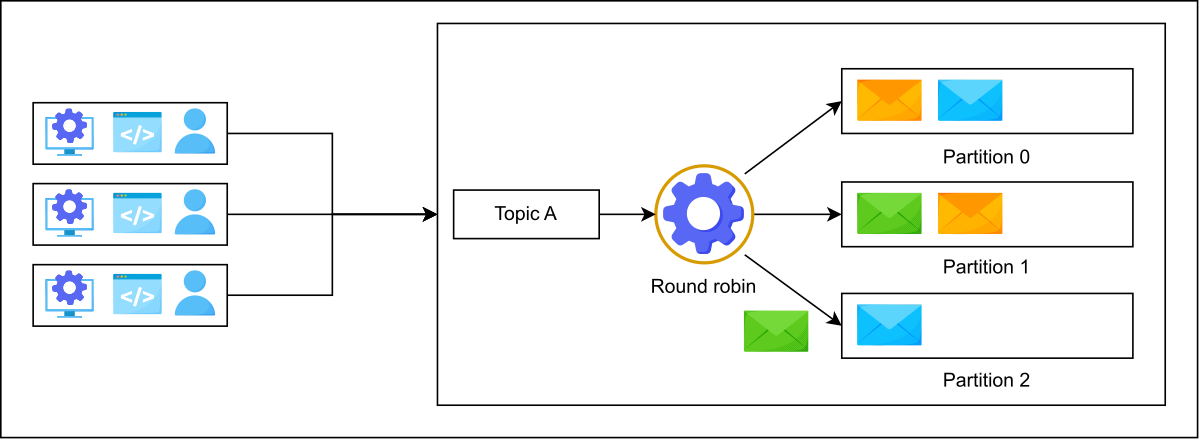
\includegraphics[width=\textwidth]{Images/chapter_18/section_5367894619193344/6536186366918656.png}
 \caption{The round-robin algorithm sends the message to Partition 2 and decides the partition for the incoming message.}
 \end{subfigure}
\end{figure}

\begin{figure}[htbp]
 \centering
 \begin{subfigure}[b]{0.48\textwidth}
 \centering
 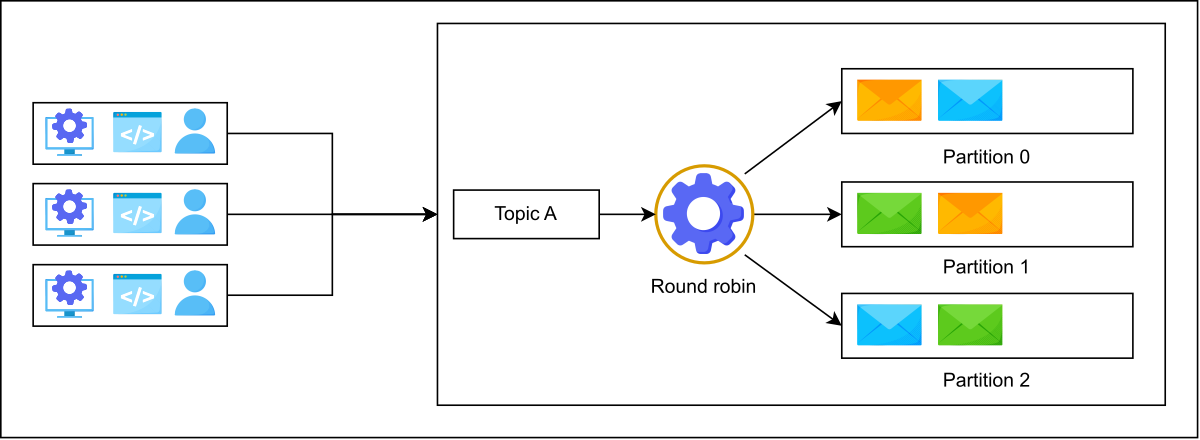
\includegraphics[width=\textwidth]{Images/chapter_18/section_5367894619193344/5100960096845824.png}
 \caption{The messages are added to the relative partitions.}
 \end{subfigure}
\end{figure}

\begin{quote}
\textbf{Quiz:}
\textbf{Question 1:} Strict ordering ensures that the messages are stored in the order in which they are produced. How can we ensure strict ordering for our messages?
\textbf{Answer:} We'll assign each partition a unique ID, `partition\_ID`. The user can provide the `partition\_ID` while writing into the system. In this way,

the messages will be sent to the specified partition, and the ordering will be strict. Our API call to write into the pub-sub system looks like this: ```txt write(topic\_ID, partition\_ID, message) ``` If the user does not provide the `partition\_ID`, we'll use the weighted round-robin algorithm to decide which message has to be sent to which partition. It might seem strange to give the ability to choose a partition to the client of pub-sub. However, such a facility can be the basis from where clients can get data for some specific time period---for example, getting data from yesterday. For simplicity, we won't include time-based reading in our design.
\textbf{Question 2:} What problems can arise if all partitions are on the same broker?
\textbf{Answer:} If the broker fails or dies, all the messages in the partitions will be lost. To avoid this, we need to make sure that the partitions are spread on different brokers.
\textbf{Question 3:} Why can't we use blob stores like S3 to keep messages, instead of the broker's local storage?
\textbf{Answer:} Blob stores like S3 are not optimized for writing and reading short-sized data. If our data is geo-replicated, the above problem is exacerbated. Therefore, we used the server's local persistent store with append-based writing. Traditional hard disks are specially tuned to provide good write performance with writing to contiguous tracks or sectors. Reading throughput and latency is also good for contiguous regions of the disk because it allows extensive data caching.
\textbf{Question 4:} If we use a round-robin algorithm to send messages to a partition, how does the system know where to look when it is time to read?
\textbf{Answer:} Our system will need to keep appropriate metadata persistently. This metadata will keep mappings between the logical index of segment or messages to the server identity or partition identifier. We'll discuss consumer manager later in the lesson, which will keep the required information.
\end{quote}

We'll allocate the partitions to various brokers in the system. This just means that different partitions of the same topic will be in different brokers. We 'll follow strict ordering in partitions by adding newer content at the end of existing messages.
\\
Consider the slides below. We have various brokers in our system. Each broker has different topics. The topic is divided into multiple partitions.

\begin{figure}[htbp]
 \centering
 \begin{subfigure}[b]{0.48\textwidth}
 \centering
 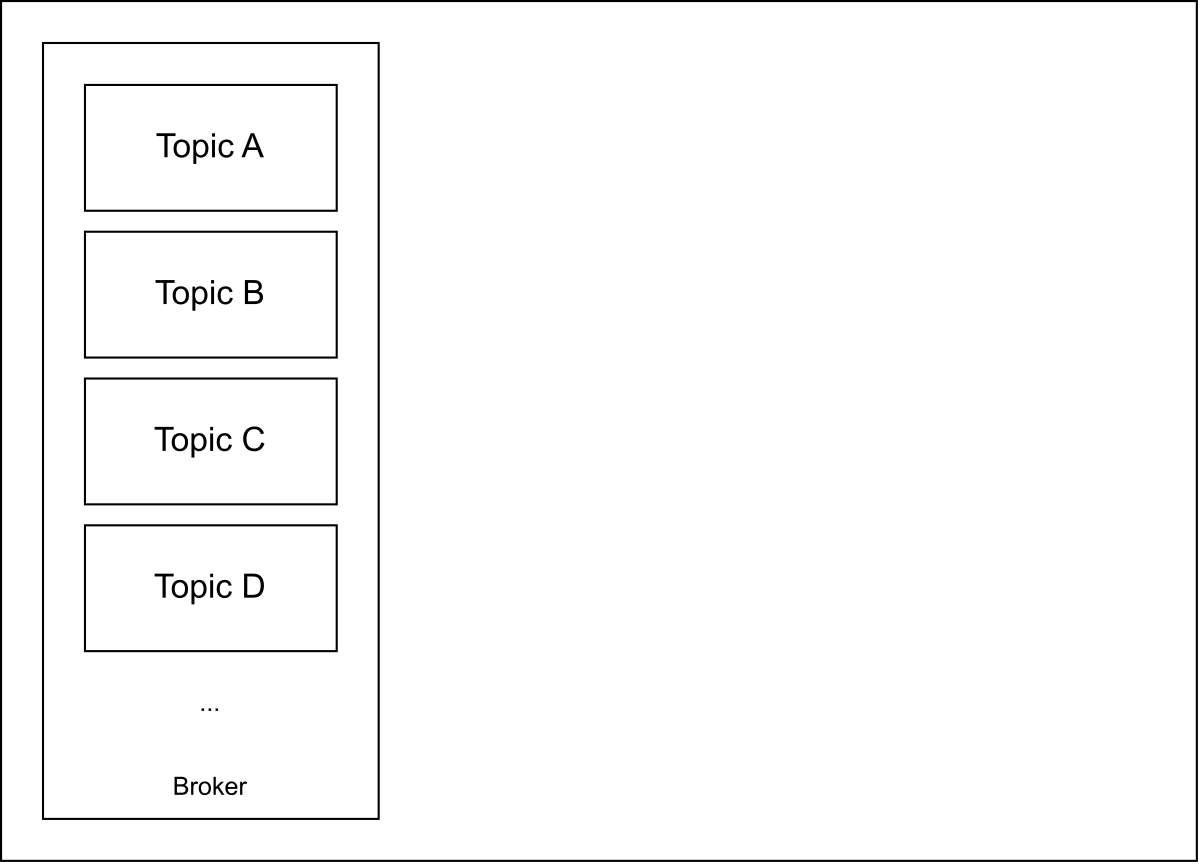
\includegraphics[width=\textwidth]{Images/chapter_18/section_5367894619193344/4932283335573504.png}
 \caption{A broker contains multiple topics.}
 \end{subfigure}
 \hfill
 \begin{subfigure}[b]{0.48\textwidth}
 \centering
 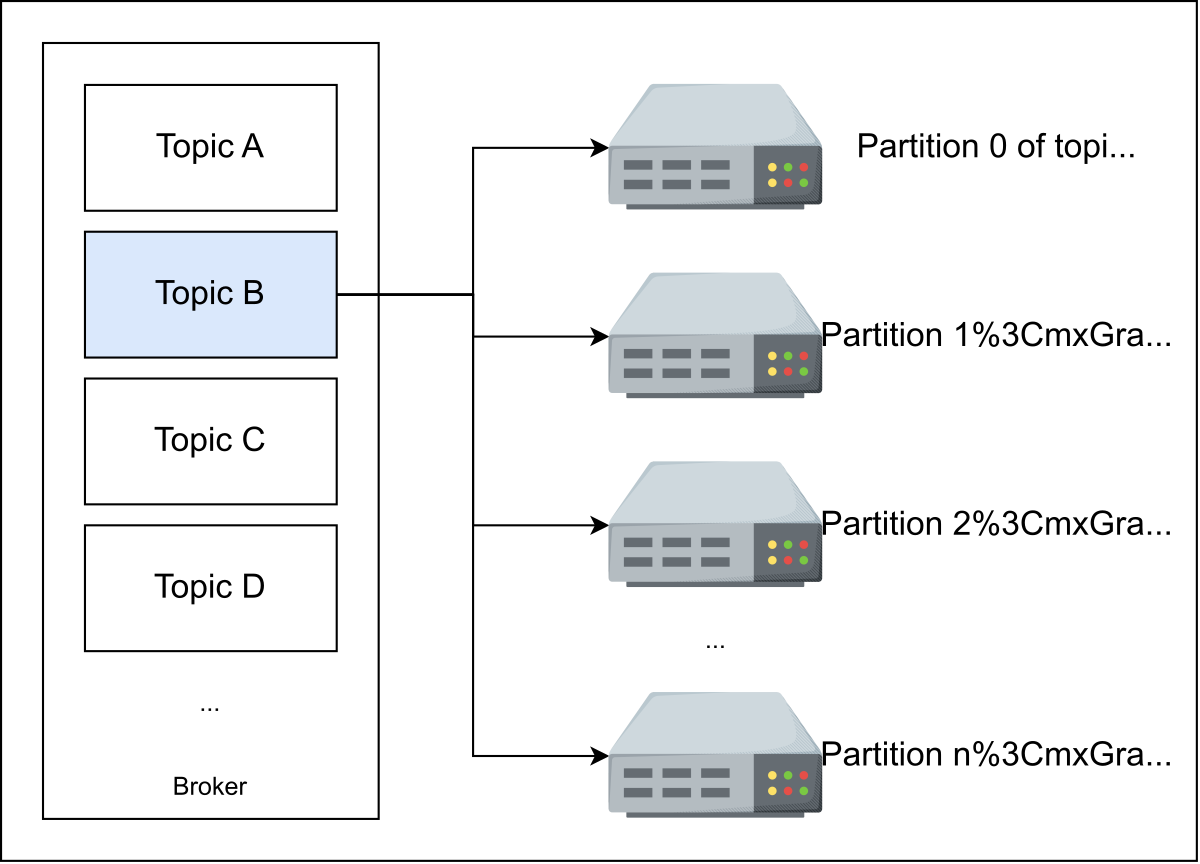
\includegraphics[width=\textwidth]{Images/chapter_18/section_5367894619193344/5364538944126976.png}
 \caption{Physical view: A topic is split into numerous partitions that are stored on other brokers.}
 \end{subfigure}
\end{figure}

\begin{figure}[htbp]
 \centering
 \begin{subfigure}[b]{0.48\textwidth}
 \centering
 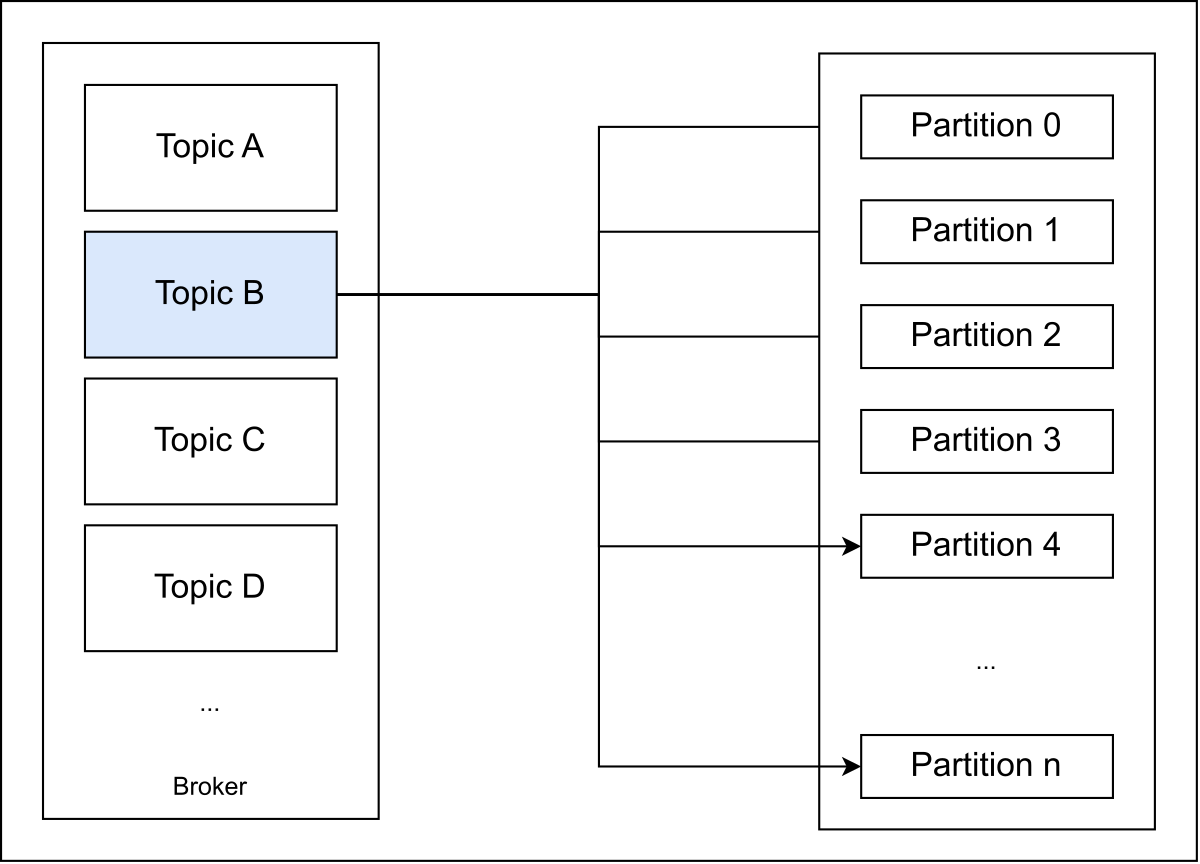
\includegraphics[width=\textwidth]{Images/chapter_18/section_5367894619193344/5539738008551424.png}
 \caption{Logical view: We can represent the partitions in another way. Here, Topic B is split into multiple partitions.}
 \end{subfigure}
\end{figure}

We discussed that a message will be stored in a segment. We'll identify each segment using an offset. Since these are immutable records, the readers are independent and they can read messages anywhere from this file using the necessary API functions. The following slides show the segment level detail.

\begin{figure}[htbp]
 \centering
 \begin{subfigure}[b]{0.48\textwidth}
 \centering
 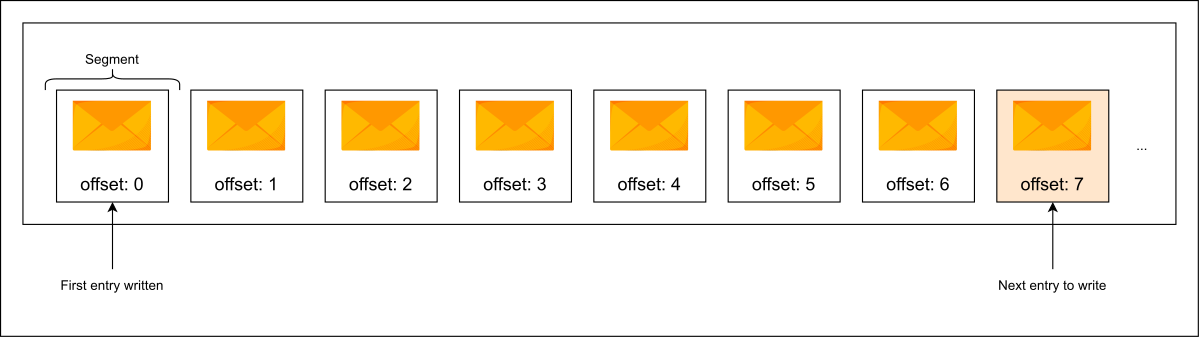
\includegraphics[width=\textwidth]{Images/chapter_18/section_5367894619193344/4959383723573248.png}
 \caption{A new entry will be added at the end of the file.}
 \end{subfigure}
 \hfill
 \begin{subfigure}[b]{0.48\textwidth}
 \centering
 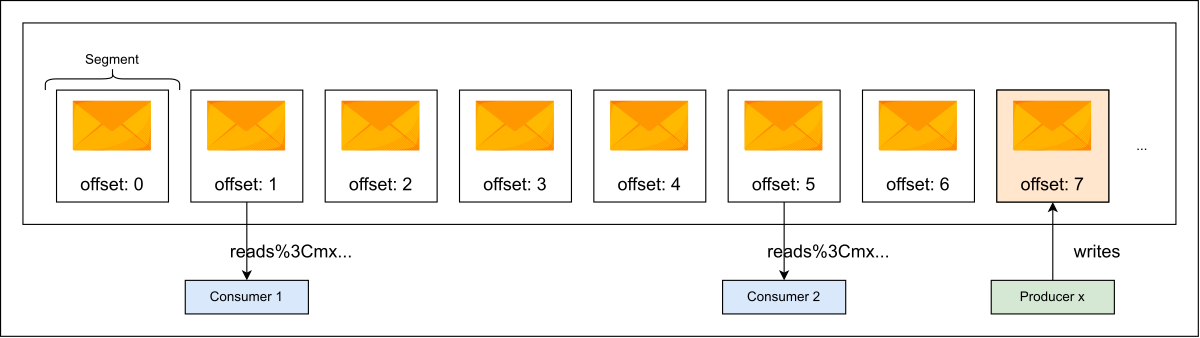
\includegraphics[width=\textwidth]{Images/chapter_18/section_5367894619193344/4781623701012480.png}
 \caption{The consumers can read anywhere from the file. Producers add to the end of file.}
 \end{subfigure}
\end{figure}

The broker solved the problems that our first design had. We avoided a large number of queues by partitioning the topic. We introduced parallelism using partitions that avoided bottlenecks while consuming the message.
\\
How would you design a pub-sub system to ensure consumers receive messages in the correct order, even when subscribing to multiple topics or partitions, assuming messages have different time stamps?\\
\\
Use the AI assessment widget below to submit your solution and get an interactive response.

\textbf{Question:}

How do we ensure message order in a pub-sub?

\textbf{Reference Answer:}

To ensure consumers receive messages in the correct order, even with multiple topics, partitions, and varying timestamps:

\begin{enumerate}
\def\labelenumi{\arabic{enumi}.}
\tightlist
\item
Partitioning strategy: Assign each topic to its own partition, ensuring ordered message delivery within each partition.

\item
Timestamp-based ordering: Include timestamps in each message and have consumers process messages based on these timestamps to maintain global order across partitions or topics.

\item
Handling multiple topics: Maintain separate consumer queues for each topic, or merge queues while respecting timestamps to preserve order across topics.

\item
Cross-partition synchronization: Use a coordinator system to track and synchronize message order across multiple partitions based on timestamps.
\end{enumerate}

\\
This approach ensures correct message ordering in a system with multiple topics and partitions.

\subsection{Cluster manager}\label{gxXG3aFplD-aoTzLup5z7}
\\
We'll have multiple brokers in our cluster. The cluster manager will perform the following tasks:

\begin{itemize}
\item
\protect\phantomsection\label{aQdgy9eJDTzECY2v4u3Cz}
\textbf{Broker and topics registry}: This stores the list of topics for each broker.
\item
\protect\phantomsection\label{NcYzr2rR1pBcZasM5RQyB}
\textbf{Manage replication}: The cluster manager manages replication by using the leader-follower approach. One of the brokers is the leader. If it fails, the manager decides who the next leader is. In case the follower fails, it adds a new broker and makes sure to turn it into an updated follower. It updates the metadata accordingly. We'll keep three replicas of each partition on different brokers.
\item
\protect\phantomsection\label{FKGZRz-etQXNIZT35QW3c}
\textbf{Authorization}: The cluster manager handles authorization for broker and topic access, as well as controlling message replication across clusters.
\end{itemize}

\begin{figure}[htbp]
 \centering
 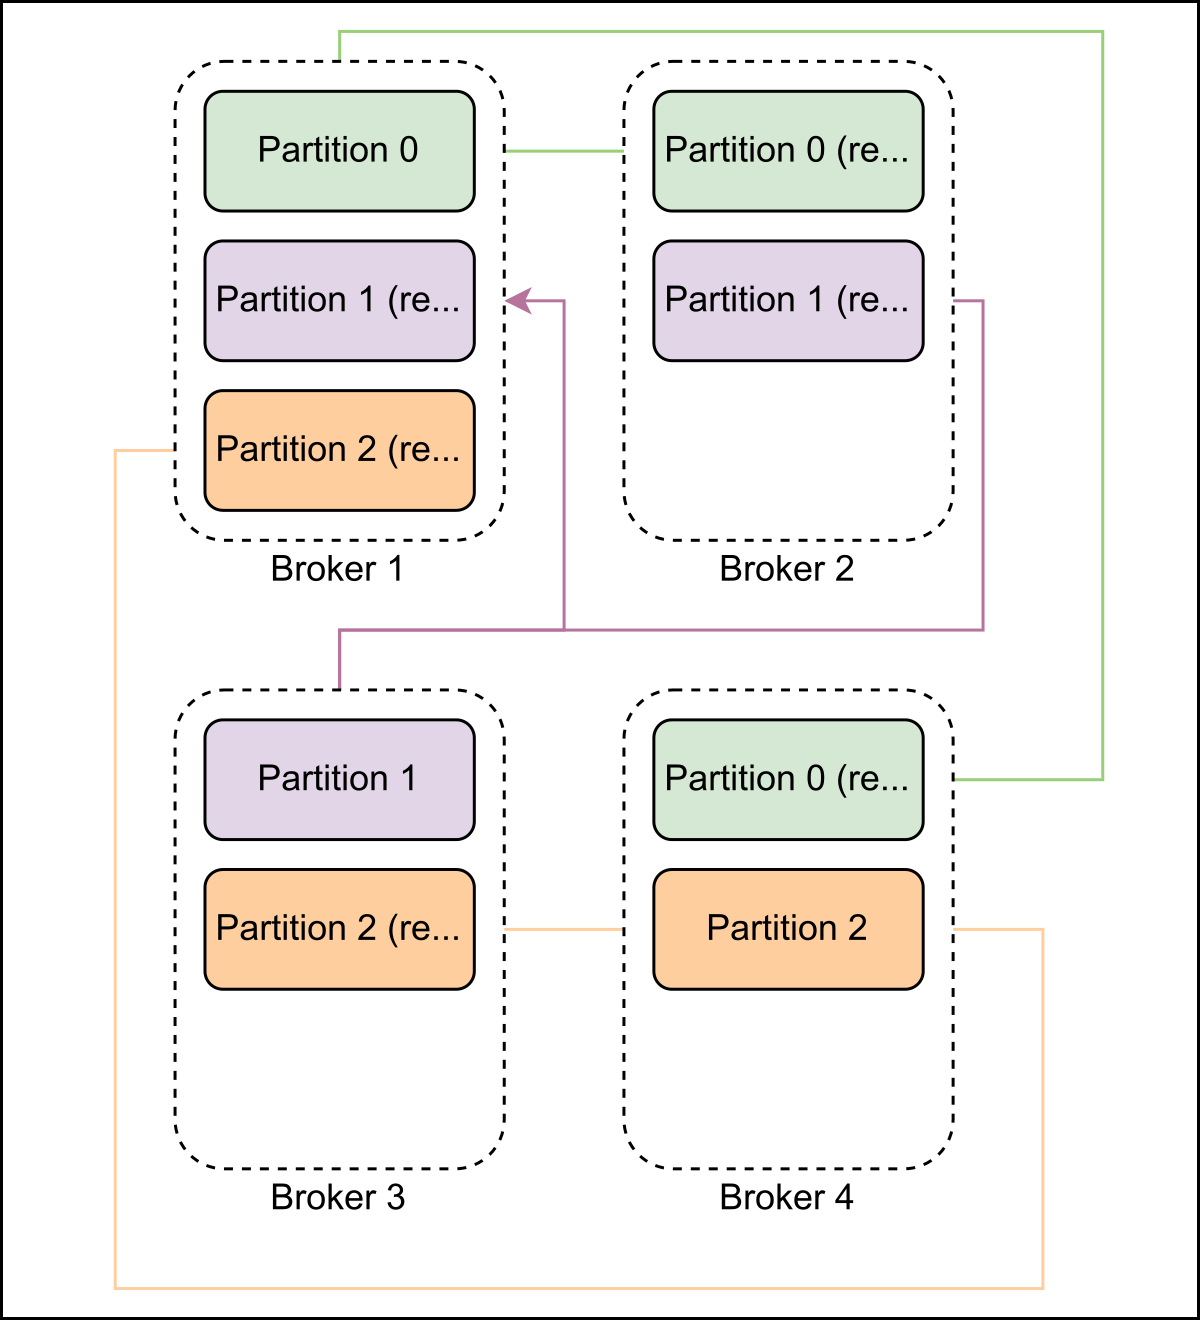
\includegraphics[width=0.5\textwidth]{Images/chapter_18/section_5367894619193344/6565408551469056.png}
 \caption{Replication at the partitioning level}
\end{figure}

\subsection{Consumer manager}\label{EUaoAyBs2JPsvz-1BPxS4}
\\
The consumer manager will manage the consumers. It has the following responsibilities:

\begin{itemize}
\item
\protect\phantomsection\label{IZ13kZqn0Zxhd6Z8wkE1v}
\textbf{Verify the consumer}: The manager will fetch the data from the database and verify if the consumer is allowed to read a certain message. For example, if the consumer has subscribed to Topic A (but not to Topic B), then it should not be allowed to read from Topic B. The consumer manager verifies the consumer's request.
\item
\protect\phantomsection\label{ekyFi8K8vdDPmw45TY-Ix}
\textbf{Retention time management}: The manager will also verify if the consumer is allowed to read the specific message or not. If, according to its retention time, the message should be inaccessible to the consumer, then it will not allow the consumer to read the message.
\item
\protect\phantomsection\label{pLFyER4mUkr-1_w6vLQh5}
\textbf{Message receiving options management}: There are two methods for consumers to get data. The first is that our system pushes the data to its consumers. This method may result in overloading the consumers with continuous messages. Another approach is for consumers to request the system to read data from a specific topic. The drawback is that a few consumers might want to know about a message as soon as it is published, but we do not support this function. Therefore, we'll support both techniques. Each consumer will inform the broker that it wants the data to be pushed automatically or it needs the data to read itself. We can avoid overloading the consumer and also provide liberty to the consumer. We'll save this information in the relational database along with other consumer details.
\item
\protect\phantomsection\label{hsl1ziU9lzqwenJKJQwzV}
\textbf{Allow multiple reads}: The consumer manager stores the offset information of each consumer. We'll use a key-value to store offset information against each consumer. It allows fast fetching and increases the availability of the consumers. If Consumer 1 has read from offset 0 and has sent the acknowledgment, we'll store it. So, when the consumer wants to read again, we can provide the next offset to the reader for reading the message.
\end{itemize}

\subsection{Finalized design}\label{i53qhQrTNjkSy13U_Jvrg}
\\
The finalized design of our pub-sub system is shown below.

\begin{figure}[htbp]
 \centering
 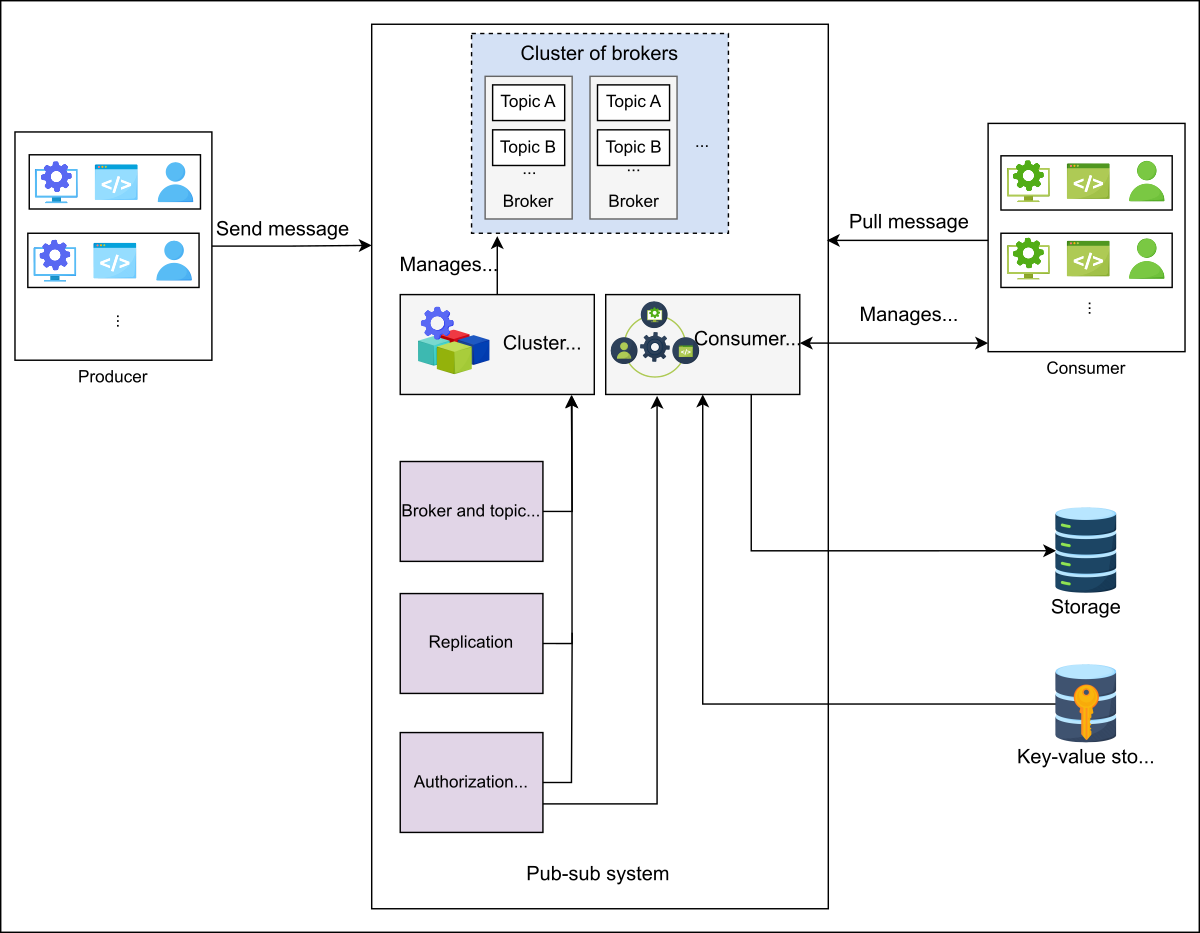
\includegraphics[width=0.5\textwidth]{Images/chapter_18/section_5367894619193344/5158341598117888.png}
 \caption{High-level design of a pub-sub system}
\end{figure}

\subsection{Conclusion}\label{O1dU-pHqUTeVIjGJty6Gl}
\\
We saw two designs of pub-sub, using queues and using our custom storage optimized for writing and reading small-sized data.
\\
There are numerous use cases of a pub-sub. Due to decoupling between producers and consumers, the system can scale dynamically, and the failures are well-contained. Additionally , due to proper accounting of data consumption, the pub-sub is a system of choice for a large-scale system that produces enormous data. We can determine precisely which data is needed and not needed.

% End of section content